\chapter{Zone d'édition}

	\section{Contrôles}

		\subsection{Déplacement}

			L'application fournis une zone d'édition relativement large. Il est possible de naviguer dans celle-ci de deux manière. Soit en utilisant les barres de navigation sur les bord la zone, soit en maintenant le clique gauche tout en déplaçant la souris.

		\subsection{Niveau de zoom}

			Il est possible d'obtenir une vue beaucoup plus générale du livre et des différents noeuds. Pour cela il suffit d'utiliser la molette de la souris.

	\section{Le prélude}

        Le prélude permet comme son nom l'indique de gérer le texte de départ du livre. Il est symbolisé par le carré fushia en haut à gauche. Cependant, celui-ci permet également de gérer deux éléments supplémentaires : La conception de la "phase de création du personnage" ainsi que l'édition du personnage principal.

		Commençons d'abord par accéder à la boite de dialogue qui permet d'ajuster les différents éléments cités précédemment. Tout d'abord, il faut sélectionner le mode 
\includegraphics[height=10pt, keepaspectratio]{img/icons/select.png}, puis double cliquer sur le prélude.

		La boite de dialogue suivante devient alors visible.

		\begin{figure}[H]
			\centering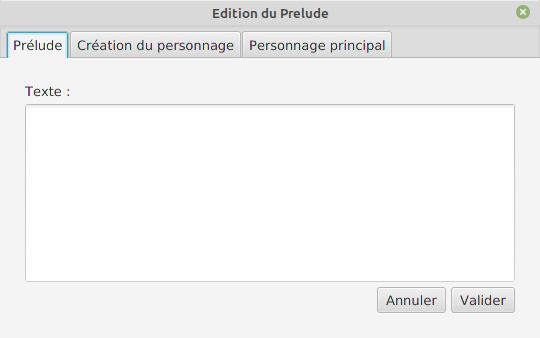
\includegraphics[width=0.4\textwidth, keepaspectratio]{img/prelude.png}
		\end{figure}

		Trois onglets sont disponibles. Le premier, "Prélude", permet de définir le texte à afficher au tout début du livre. Il permet de situer le lecteur dans l'univers de ce qu'il va lire. Le deuxième, "Création du peronnage" permet au lecteur de faire différents choix concernant son personnage, que cela soit sur les compétences qu'il possèdera, les items avec lesquels il débutera ou encore les items supplémentaires qu'il peut acheter. Et enfin, "Personnage Principal" qui permet de définir les caractéristiques de celui-ci.

		Nous ne détaillerons pas l'onglet concernant le Prélude car celui-ci est suffisement explicite.

		\subsection{Création du personnage}
			Cette onglet à un bouton 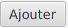
\includegraphics[height=10pt, keepaspectratio]{img/ajouterBouton.png}, permettant d'ajouter une étape, dans la conception du personnage, étape visible sur l'image ci-dessous.

			\begin{figure}[H]
				\centering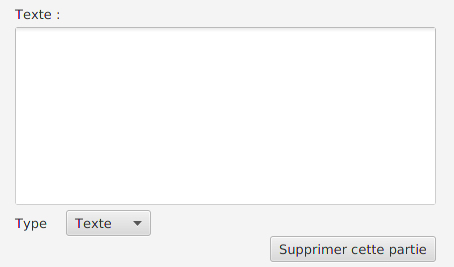
\includegraphics[width=0.4\textwidth, keepaspectratio]{img/etapeConceptionPerso.png}
			\end{figure}

			La zone de texte permet d'introduire le choix concernant le type d'élément (items, compétences, ...) que le joueur peut choisir pour son personnage tandis que la liste déroulante permet de sélectionner le type de cette étape. Il est important d'avoir déjà ajouter des items ou compétences pour voir cette liste (cf : \nameref{chapter:elementsConstitutifLivre} page \pageref{chapter:elementsConstitutifLivre}).

			Le bouton 
\includegraphics[height=10pt, keepaspectratio]{img/preludeSupprimerBouton.png} permet de supprimer l'étape.

			\subsubsection{Le type item / shop}
				\phantomsection\label{subsubsec:item_shop}

				Une liste déroulante s'affiche avec tout les items encore non sélectionné. Pour ajouter un item, il faut d'abord en sélectionner un, puis cliquer sur le bouton 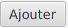
\includegraphics[height=10pt, keepaspectratio]{img/ajouterBouton.png}. Une fois l'item ajouté, il peut-être supprimé en faisant apparaitre le menu grâce à un clique droit sur celui-ci.

				L'utilisateur peut aussi le sélectionner afin de renseigner changer certaines informations :

				\begin{description}
					\item[Type Item :] Le nombre d'item disponible
					\item[Type Shop :] Le nombre d'item disponible à la vente, ainsi que son prix d'achat et son prix de revente
				\end{description}

				Si un champ est changé, l'utilisateur doit alors cliquer sur le bouton modifier pour prendre en compte les changements, ce sans quoi, ils seront simplement ignorés.

			\subsubsection{Le type compétence}
				\phantomsection \label{subsubsec:persoCreationSkill}

				Le bouton 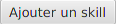
\includegraphics[height=10pt, keepaspectratio]{img/preludeAjouterSkillBouton.png} affiche une liste déroulante permettant de sélectionner la compétence que l'on souhaite rendre disponible dans le choix du joueur. Si l'on souhaite supprimer l'une des compétences il suffit de sélectionner l'élément vide et de valider les modifications sur la boite de dialogue.

		\subsection{Personnage principal}
			\label{subsec:main_character}

			L'affichage est casiment identique à celui concernant l'ajout d'un personnage basique (cf : \nameref{sec:perso} page \pageref{sec:perso}). Quelques champs supplémentaires sontt présent comme la quantité d'items pouvant être porté et la somme qu'il possède au départ.

	\section{Les noeuds}

		\label{sec:noeuds}
		La création d'un noeud se fait à partir du mode 
\includegraphics[height=10pt, keepaspectratio]{img/icons/add_node.png}. Ce mode permet de créer un paragraphe d'un simple clique sur la zone d'édition. Une boite de dialogue proposant diverses choix dans le type de noeuds.

		\subsection{Champs communs}

			Chaque noeud possède une zone de texte permettant d'entrer le texte du paragraphe. Les noeuds de victoire et de défaite ne possède pas d'autres champs ou onglets que celui-ci. Outre cette zone de texte, trois onglets sont égalements présent (sauf pour les noeuds de victoire et de défaite donc) : l'un permettant l'édition du noeud (\textit{Noeud}), l'autre l'ajout des items à prendre (\textit{Item}), et le dernier, l'ajout d'items achetetable (\textit{Shop}). Bien évidemment, pour sélectionner des items dans ces deux derniers onglets, il faut au préalable en avoir ajouté.

			De plus les noeuds possèdent deux champs supplémentaires, l'un permettant de renseigner le montant de PV à gagner / perdre, l'autre permettant de sélectionner le nombre maximum d'items pouvant être pris dans parmis ceux sélectionnés dans l'onglet \textit{Item}. Si ce nombre vaut -1, alors on peut prendre autant d'item que l'on veut.

			\subsubsection{Noeud basic}

				Ce type de noeud ne possède aucun champ suplémentaire. Il s'agit d'un simple paragraphe avec une liste de choix.

			\subsubsection{Noeud aléatoire}

				Ce noeud ne diffère pas du noeud "basic sur sa présentation. Cependant,lors de la création des liens, certaines informations supplémentaires seront disponibles (cf : \nameref{subsubsec:lienAléatoire} page \pageref{subsubsec:lienAléatoire}).

			\subsubsection{Noeud combat}
				\phantomsection\label{subsubsec:combat}

				Ce noeud contient deux nouvelles données à remplir. Tout d'abord, il est possible de définir le nombre de tours avant de pouvoir s'évader. Puis il y a un bouton 
\includegraphics[height=10pt]{img/noeudAddPersonnage} permettant d'ajouter des ennemis grâce à la liste déroulante qui apparait. Chaque ennemis peut être ajouté plusieurs fois, par exemple, dans le but de créer une horde de zombie. Bien évidemment, pour choisir un ennemi, il faut d'abord avoir saisie des personnages (cf : \nameref{sec:perso} à la page \pageref{sec:perso})

				Des éléments supplémentaires seront disponibles sur liens lors de la création de ceux-ci (cf : \nameref{subsubsec:lienCombat} page \pageref{subsubsec:lienCombat}).

			\subsubsection{Noeud Victoire / Défaite}

				Ces noeuds permettent de définir si le joueur a gagné ou perdu. Le livre est donc fini à cette endroit. Ces noeuds ne peuvent bien entendu pas contenir de choix.

		\subsection{Modification des noeuds}

			Pour modifier un noeud, il faut d'abord sélectionner le mode 
\includegraphics[height=10pt, keepaspectratio]{img/icons/select.png}, puis double cliquer le noeud à modifier. Attention, si l'on change le type d'un noeud et que des liens étaient présent suur celui-ci, ils sont tout simplement supprimés.

		\subsection{Positionnement des noeuds}

			Les noeuds peuvent être déplacés grâce au mode 
\includegraphics[height=10pt]{img/icons/select.png}. Le simple fait de glisser la souris tout en maintenant le clique gauche depuis un noeud suffit pour le déplacer.

		\subsection{Supression des noeuds}

			Tous les noeuds, peuveut être supprimés à l'aide du mode 
\includegraphics[height=10pt, keepaspectratio]{img/icons/delete.png}. Un simple clique sur le noeud permet de réaliser cette action qui nécessite confirmation. Attention, si des liens étaient présent sur ce noeud, ils sont tout simplement supprimés.

	\section{Lier les éléments}
		\label{sec:lien}

		\subsection{Désigner le premier noeud}

			Cela permet d'indiquer le premier noeud qui va être lu, après le prélude. Ce lien est donc très important car il permet d'utiliser toutes les options possible dans l'onglet "\textit{Livre}" de la barre de menu. Ce lien peut être réalisé grâce au mode 
\includegraphics[height=10pt, keepaspectratio]{img/icons/first_node.png} même si le prélude ainsi que d'un simple clique sur le noeud que l'on souhaite désigner comme étant le premier.

		\subsection{Lien entre les noeuds}

			Ces liens permettent de relier un paragraphe à un autre paragraphe par l'intermédiaire d'un choix. Ces liens étant dirigé, c'eest à dire que l'on passe d'un noeud à n'autre sans possibilité de revenir, ils ne peuvent donc pas commencer sur un noeud de défaite / victoire ou sur le prélude.

			Pour tracer ce lien, le mode 
\includegraphics[height=10pt, keepaspectratio]{img/icons/add_link.png} est requis. L'utilisateur doit alors cliquer sur un premier noeud (noeud source), puis sur un deuxième (noeud de destination). Ce noeud peut être le même afin de laisser la liberté de créer une boucle si necessaire. Cependant il sera difficile de l'éditer ou de le supprimer par la suite. Cette même difficulté est présente si l'on souhaite faire en sorte de pouvoir revenir au noeud précédent, les deux noeuds seront superposés. Si le permier clique n'était pas voulu, un simple clique dans la zone vide d'édition permet d'annulé la sélection faite.

			Une fois les deux noeuds sélectionnés, une boite de dialog apparait. Elle contient un texte qui décrit le choix, deux champs de texte de gain/perte de point de vie et de monnaie, ainsi que d'un onglet contenant les prérequis. Une case est également disponible permettant de toujours ce choix automatiquemenent si on remplis tous les prérequis.

			\subsubsection{Les prérequis}
				\phantomsection\label{sec:prerequis}

				Ces prérequis permettent à l'utilisateur de créer des choix qu'il est possible d'entreprendre que si certains objets / compétences / une certaine somme d'argent est possédés par le joueur. Par exemple, le joueur doit posséder l'épée "Excalibur" ainsi que le bouclier "Pavois" \textbf{ou} trois d'argent ainsi que la compétence "Boule de feu" et l'épée "Excalibur". Pour cela, un bouton 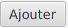
\includegraphics[height=10pt, keepaspectratio]{img/ajouterBouton.png} permet de créer une liste de prérequis dans laquel le joueur doit posséder \textbf{tous les éléments en même temps}. Pour faire un autre ensemble de condiion, il faut refaire une nouvelle liste.
				Pour l'ajout de ces items / monnaie / compétences, c'est le même procédé que \nameref{sec:skills} et \ref{subsubsec:item_shop}.

			\subsubsection{Lien noeud combat}
				\phantomsection\label{subsubsec:lienCombat}

				\begin{wrapfigure}{r}{4cm}
					\centering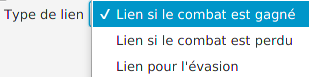
\includegraphics[width=4cm, keepaspectratio]{img/lienCombat.png}
				\end{wrapfigure}
				Si le premier noeud cliqué est un noeud de combat, une liste déroulante "Type de lien" est présente dans l'onglet lien. Ce type permet de savoir dans quel condition le choix sera pris (victoire, défaite, évasion). Il est important de noter que si le lien de victoire n'est pas définit, le jeu considérera que le joueur a perdu.

			\subsubsection{Lien noeud aléatoire}
				\phantomsection\label{subsubsec:lienAléatoire}

				Si le premier noeud cliqué est un noeud aléaoire, un champ de texte permet de renseigner la probabilité que ce lien soit choisit.

				\begin{figure}[H]
					\centering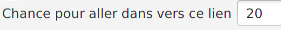
\includegraphics[width=0.4\textwidth, keepaspectratio]{img/lienAleatoire.png}
				\end{figure}

		\subsection{Modification des liens}

			Une modification des liens se fait grâce au mode 
\includegraphics[height=10pt, keepaspectratio]{img/icons/select.png}. Un simple double clique sur le lien est necessaire pour modifier ce dernier.

		\subsection{Suppression des liens}

			Ces liens, sauf celui avec le prélude, peuveut être supprimés à l'aide du mode 
\includegraphics[height=10pt, keepaspectratio]{img/icons/delete.png}. Un simple clique sur le lien permet de réaliser cette action qui nécessite confirmation. Si le lien concernait un lien ur un noeud de combat, le type de ce lien est alors libre.
